\section{Natural Language Toolkit (NLTK)}

NLTK\footnote{\href{http://www.nltk.org/}{NLTK: http://www.nltk.org/}} ist eine Python Bibliothek um natürliche Sprache zu verarbeiten.
Dabei nutzen wir die Funktionen zur Klassifizierung der einzelnen
Textbausteine. Dabei liefert NLTK eine Liste von Paaren, die den
kompletten Text als einzelne Tokens mit ihrer gegebenen
Klassifizierung darstellt.

Zum Klassifizieren bietet NLTK eine vielzahl von Algorithmen an, wir
verwenden für unsere Untersuchung den \textit{BrillTagger}, da dieser
laut Dokumentation eine sehr gute Erkennunsrate aufweist.

\section{Hearst Patterns}

Hearst Patterns werden verwendet um \textit{Hyponyme} für ein gegebenes
\textit{Hypernym} zu finden. Dabei gelten folgende Regeln
$$R \subseteq M \times M$$
$$\forall x, y, z \in M : xRy \land yRz \Rightarrow xRz$$
$$\forall x \in M : \neg xRx$$
$$\forall x, y \in M : xRy \Rightarrow \neg (yRx)$$%
%
wobei $M$ die Menge aller Wörter der entsprechenden Sprache ist.
% TODO Quelle hinzufügen (aktuell Wikipedia ~> dort keine Quelle
% angegben -.-)

Um die entsprechenden Hyponyme in einem Corpus zu finden, werden
bestimmte Muster in Texten gesucht, die folgende Liste zeigt die
verwendeten Patterns, dabei ist $NP_{X}$ das Hyponym und $NP_{Y}$ das
dazugehörige Hypernym.

\begin{itemize}
\item $NP_{X}$ and other $NP_{Y}$
\item $NP_{X}$ or other $NP_{Y}$
\item $NP_{Y}$ such as $NP_{X}$
\item Such $NP_{Y}$ as $NP_{X}$
\item $NP_{Y}$ including $NP_{X}$
\item $NP_{Y}$, especially $NP_{X}$
\end{itemize}%
%
So können Hyponyme zu entsprechenden Hypernymen gefunden werden.
\cite{Snow:2004}

In unserer
Implementierung\footnote{\href{https://github.com/tbraun89/research-textmining}{Github:
 https://github.com/tbraun89/research-textmining}} verwenden wir einen deterministischen
Automaten (DFA), der als Eingabe die Liste von Paaren des Textes
erhällt und so in einer Laufzeit von $\mathcal{O}(n)$ alle Beziehungen
findet. Die Ergebnisse des DFA werden dann in einer Datei gespeichert
um weitere Untersuchungen damit durchführen zu können.
~\\~\\

\begin{centering}
  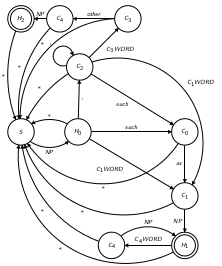
\includegraphics[scale=0.75]{img/hpdfa}
\end{centering}

\section{Aktuelle Ergebnisse}

Für die aktuelle Untersuchung haben wir den \textit{Open American
National Corpus} (ONAC) verwendet. Dieser besteht aus 11.939.180 
Wörtern. Mit unserem DFA konnten wir nach der Klassifizierung durch
NLTK 2.716 Hypernyme mit 21.028 Hyponymen erkennen.

An den Gefundenen Daten kann man erkennen, dass die Qualität der
gefundenen Beziehungen in nur ca. 50\% der Ergebnisse korrekt ist. Es
werden auch sehr viele Beziehungen gefunden, die zwar den Patterns
entsprechen, allerdings sprachlich keine Beziehungen sind. Dies zeigt,
das rein die Verwendung von Hearst Patterns nicht ausreicht, um
Hypernym- und Hyponymbeziehungen in Texten zu erkennen und eine
nachträgliche Selektierung der Ergebnisse notwendig ist.
